% Template for PLoS
% Version 3.1 February 2015
%
% To compile to pdf, run:
% latex plos.template
% bibtex plos.template
% latex plos.template
% latex plos.template
% dvipdf plos.template
%
% % % % % % % % % % % % % % % % % % % % % %
%
% -- IMPORTANT NOTE
%
% This template contains comments intended
% to minimize problems and delays during our production
% process. Please follow the template instructions
% whenever possible.
%
% % % % % % % % % % % % % % % % % % % % % % %
%
% Once your paper is accepted for publication,
% PLEASE REMOVE ALL TRACKED CHANGES in this file and leave only
% the final text of your manuscript.
%
% There are no restrictions on package use within the LaTeX files except that
% no packages listed in the template may be deleted.
%
% Please do not include colors or graphics in the text.
%
% Please do not create a heading level below \subsection. For 3rd level
% headings, use \paragraph{}.
%
% % % % % % % % % % % % % % % % % % % % % % %
%
% -- FIGURES AND TABLES
%
% Please include tables/figure captions directly after the paragraph where they
% are first cited in the text.
%
% DO NOT INCLUDE GRAPHICS IN YOUR MANUSCRIPT
% - Figures should be uploaded separately from your manuscript file.
% - Figures generated using LaTeX should be extracted and removed from the PDF
% before submission.
% - Figures containing multiple panels/subfigures must be combined into one
% image file before submission.
% For figure citations, please use "Fig." instead of "Figure".
% See http://www.plosone.org/static/figureGuidelines for PLOS figure guidelines.
%
% Tables should be cell-based and may not contain:
% - tabs/spacing/line breaks within cells to alter layout or alignment
% - vertically-merged cells (no tabular environments within tabular
% environments, do not use \multirow)
% - colors, shading, or graphic objects
% See http://www.plosone.org/static/figureGuidelines#tables for table
% guidelines.
%
% For tables that exceed the width of the text column, use the adjustwidth
% environment as illustrated in the example table in text below.
%
% % % % % % % % % % % % % % % % % % % % % % % %
%
% -- EQUATIONS, MATH SYMBOLS, SUBSCRIPTS, AND SUPERSCRIPTS
%
% IMPORTANT
% Below are a few tips to help format your equations and other special
% characters according to our specifications. For more tips to help reduce the
% possibility of formatting errors during conversion, please see our LaTeX
% guidelines at http://www.plosone.org/static/latexGuidelines
%
% Please be sure to include all portions of an equation in the math environment.
%
% Do not include text that is not math in the math environment. For example, CO2
% will be CO\textsubscript{2}.
%
% Please add line breaks to long display equations when possible in order to fit
% size of the column.
%
% For inline equations, please do not include punctuation (commas, etc) within
% the math environment unless this is part of the equation.
%
% % % % % % % % % % % % % % % % % % % % % % % %
%
% Please contact latex@plos.org with any questions.
%
% % % % % % % % % % % % % % % % % % % % % % % %

\documentclass[10pt,letterpaper]{article}
\usepackage[top=0.85in,left=2.75in,footskip=0.75in]{geometry}

% Use adjustwidth environment to exceed column width (see example table in text)
\usepackage{changepage}

% Use Unicode characters when possible
\usepackage[utf8]{inputenc}

% textcomp package and marvosym package for additional characters
\usepackage{textcomp,marvosym}

% fixltx2e package for \textsubscript
\usepackage{fixltx2e}

% amsmath and amssymb packages, useful for mathematical formulas and symbols
\usepackage{amsmath,amssymb}

% cite package, to clean up citations in the main text. Do not remove.
\usepackage{cite}

% Use nameref to cite supporting information files (see Supporting Information
% section for more info)
\usepackage{nameref,hyperref}

% line numbers
\usepackage[right]{lineno}

% ligatures disabled
\usepackage{microtype}
\DisableLigatures[f]{encoding = *, family = * }

% rotating package for sideways tables
\usepackage{rotating}

% Remove comment for double spacing
%\usepackage{setspace} 
%\doublespacing

% Text layout
\raggedright
\setlength{\parindent}{0.5cm}
\textwidth 5.25in 
\textheight 8.75in

% Bold the 'Figure #' in the caption and separate it from the title/caption with
% a period
% Captions will be left justified
\usepackage[aboveskip=1pt,labelfont=bf,labelsep=period,justification=raggedright,
singlelinecheck=off]{caption}

% Use the PLoS provided BiBTeX style
\bibliographystyle{plos2015}

% Remove brackets from numbering in List of References
\makeatletter
\renewcommand{\@biblabel}[1]{\quad#1.}
\makeatother

% Leave date blank
\date{}

% Header and Footer with logo
\usepackage{lastpage,fancyhdr,graphicx}
\usepackage{epstopdf}
\pagestyle{myheadings}
\pagestyle{fancy}
\fancyhf{}
\lhead{\includegraphics[width=2.0in]{PLOS-submission.eps}}
\rfoot{\thepage/\pageref{LastPage}}
\renewcommand{\footrule}{\hrule height 2pt \vspace{2mm}}
\fancyheadoffset[L]{2.25in}
\fancyfootoffset[L]{2.25in}
\lfoot{\sf PLOS}

%% Include all macros below

\newcommand{\lorem}{{\bf LOREM}}
\newcommand{\ipsum}{{\bf IPSUM}}

%% END MACROS SECTION


\begin{document}
\vspace*{0.35in}

% Title must be 250 characters or less.
% Please capitalize all terms in the title except conjunctions, prepositions,
% and articles.
\begin{flushleft}
{\Large
\textbf\newline{Article Title - Submission to PLOS Journals}
}
\newline
% Insert author names, affiliations and corresponding author email (do not include 
% titles, positions, or degrees).
\\
Name1 Surname\textsuperscript{1,\Yinyang},
Name2 Surname\textsuperscript{2,\Yinyang},
Name3 Surname\textsuperscript{2,\textcurrency a},
Name4 Surname\textsuperscript{2,\ddag},
Name5 Surname\textsuperscript{2,\ddag},
Name6 Surname\textsuperscript{2},
Name7 Surname\textsuperscript{3,*},
with the Lorem Ipsum Consortium\textsuperscript{\textpilcrow}
\\
\bigskip
\bf{1} Affiliation Dept/Program/Center, Institution Name, City, State, Country
\\
\bf{2} Affiliation Dept/Program/Center, Institution Name, City, State, Country
\\
\bf{3} Affiliation Dept/Program/Center, Institution Name, City, State, Country
\\
\bigskip

% Insert additional author notes using the symbols described below. Insert
% symbol callouts after author names as necessary.
%
% Remove or comment out the author notes below if they aren't used.
%
% Primary Equal Contribution Note
\Yinyang These authors contributed equally to this work.

% Additional Equal Contribution Note
% Also use this double-dagger symbol for special authorship notes, such as
% senior authorship.
\ddag These authors also contributed equally to this work.

% Current address notes
\textcurrency a Insert current address of first author with an address update
% \textcurrency b Insert current address of second author with an address update
% \textcurrency c Insert current address of third author with an address update

% Deceased author note
\dag Deceased

% Group/Consortium Author Note
\textpilcrow Membership list can be found in the Acknowledgments section.

% Use the asterisk to denote corresponding authorship and provide email address in note below.
* CorrespondingAuthor@institute.edu

\end{flushleft}

% Please keep the abstract below 300 words
\section*{Abstract}

Lorem ipsum dolor sit amet, consectetur adipiscing elit. Curabitur eget porta
erat. Morbi consectetur est vel gravida pretium. Suspendisse ut dui eu ante
cursus gravida non sed sem. Nullam sapien tellus, commodo id velit id, eleifend
volutpat quam. Phasellus mauris velit, dapibus finibus elementum vel, pulvinar
non tellus. Nunc pellentesque pretium diam, quis maximus dolor faucibus id. Nunc
convallis sodales ante, ut ullamcorper est egestas vitae. Nam sit amet enim
ultrices, ultrices elit pulvinar, volutpat risus.


% Please keep the Author Summary between 150 and 200 words
% Use first person. PLOS ONE authors please skip this step. 
% Author Summary not valid for PLOS ONE submissions.   
\section*{Author Summary}
Lorem ipsum dolor sit amet, consectetur adipiscing elit. Curabitur eget porta
erat. Morbi consectetur est vel gravida pretium. Suspendisse ut dui eu ante
cursus gravida non sed sem. Nullam sapien tellus, commodo id velit id, eleifend
volutpat quam. Phasellus mauris velit, dapibus finibus elementum vel, pulvinar
non tellus. Nunc pellentesque pretium diam, quis maximus dolor faucibus id. Nunc
convallis sodales ante, ut ullamcorper est egestas vitae. Nam sit amet enim
ultrices, ultrices elit pulvinar, volutpat risus.

\linenumbers

\section*{Introduction}
Sandia National Laboratory (SNL) developed the cross-flow turbine, Reference
Model 2 (RM2), to provide an open-source point design for MHK research and
development, including its use as a test object for scaled model testing to
generate power performance data that can be used to validate open-source design
tools. More details on the reference modeling effort are provided in Neary et
al. \cite{Neary2014}.

Dimensional analysis provides scaling laws that are used to upscale model test
data into performance and design information for a full-scale prototype turbine.
For hydrokinetic turbines, hydrodynamic similitude is achieved when the Reynolds
number, Froude number and tip-speed-ratio of the model and the full scale device
match. The Reynolds number is defined as
\begin{equation}
Re_L = \frac{UL}{\nu},
\label{eq-Re}
\end{equation}
where $U$ and $L$ are characteristic length scales, and $\nu$ is the fluid
kinematic viscosity. The Froude number is defined as
\begin{equation}
Fr = \frac{U}{\sqrt{gL}},
\label{eq-Fr}
\end{equation}
where $g$ is the gravitational acceleration, and the tip speed ratio is defined
as
\begin{equation}
\lambda=\frac{\omega R}{U_\infty},
\end{equation}
where $\omega$ and $R$ are the rotor angular velocity and radius.
For hydrokinetic turbine testing, $Re$, not $Fr$, is the dominant scaling
parameter. However, the Froude number (based on blade tip submergence) should
remain small (significantly below one). It is rare to achieve perfect similitude
for $Re$, but a threshold value should be exceeded, such that scale model
results can be extrapolated.

As a cross-flow turbine, the RM2 blades will experience large variations in
angles of attack as they rotate about their axis (``cross-flow turbine'' means
the axis of rotation is perpendicular to flow direction---either vertically or
horizontally). These variations become larger as the tip speed ratio decreases
\cite{Para2002}. Typically, the maximum angles of attack are sufficiently large
that the blades operate under dynamic stall, which is a complex unsteady process
and deviates significantly from static foil behavior, during part of the
rotation. Furthermore, the higher the solidity of a cross-flow turbine, the
lower the optimal tip-speed ratio at which it operates. Marine Hydrokinetic
(MHK) cross-flow turbines typically have higher solidity than cross-flow wind
turbines (VAWT), and hence operate at lower tip-speed ratios. Since MHK turbines
operate in a higher density fluid, unsteady dynamic effects related to the
blades' pitching motion and flow curvature also become more important when
compared to wind turbines.

The performance of cross-flow MHK turbines thus depends on both Reynolds number
and solidity (note that these issues are related, since an average blade chord
Reynolds number, $Re_{c,\mathrm{avg}} \approx \lambda U_\infty c/ \nu$, can be
expressed in terms of tip speed ratio, the optimal value for which is a function
of solidity). If numerical models are validated with physical model data that
was obtained at insufficiently high Reynolds numbers, it cannot be determined
whether problems with model predictions are caused by Reynolds number effects,
issues related to higher solidity, or both. It is uncertain whether numerical
models validated with physical model data obtained at low Reynolds number should
be considered validated at all, since the scale at which the model will be
applied is orders of magnitude larger. One way to overcome this uncertainty is
to show that the scaled physical model test has become Reynolds number
independent, and therefore validation efforts should be relevant at full-scale.

For example, the effect of Reynolds number on average power output was shown to
be significant on the 2 m Sandia Research Darrieus turbine in wind tunnel
testing \cite{Blackwell1976}: Maximum power coefficient, $C_{P,\mathrm{max}}$,
increased with Reynolds number, $Re_c$, along with a shift of the location of
$C_{P,\mathrm{max}}$ toward lower tip speed ratios due to delayed blade stall.
The effects of Reynolds number were quite dramatic over a relatively small range
of $Re_c \approx 1.1 \times 10^5$--$2.9 \times 10^5$. More recently, Bachant and
Wosnik \cite{Bachant2014} showed that turbine performance and near-wake
characteristics become Reynolds number independent at $Re_c \approx 2 \times
10^5$.

The need for experimental data that is relevant to full-scale behavior stems
from the need to validate numerical models---most importantly mid-fidelity
models---desirable for MHK developers to predict the performance of their
cross-flow turbine designs, since physical modeling at appropriate scales can be
prohibitively expensive in the early stages of engineering. Furthermore,
Navier--Stokes-based computational fluid dynamics (CFD) simulations require
modeling in 3 dimensions, which generally necessitates high performance
computing---a resource that is not commonly available, and more expensive.

To date, attempts to validate SNL's mid-fidelity CACTUS vortex line model
\cite{Murray2011} have relied on measurements from the Saint Anthony Falls
Laboratory (SAFL) \cite{Hill2014} and the University of New Hampshire (UNH)
\cite{Neary2013, Michelen2014}. For the SAFL experiments (RM2), the chord
Reynolds number, $Re_c \sim 10^4$, was below the threshold needed to properly
simulate lift and stall characteristics. For the UNH experiment
\cite{Bachant2013}, the chord Reynolds number was sufficiently high at $Re_c
\approx 2.7 \times 10^5$, but the chord/radius ratio and solidity (13.4\%)
created instability in the free-wake evolution in the model, which caused
significant overestimation of power coefficient.

The present task is to acquire a new dataset for the lower solidity RM2 turbine,
but at higher Reynolds numbers than those achieved in the experiments at SAFL.
It is also suspected that the strut drag model in CACTUS could be the source of
some discrepancy. The strut drag will be deliberately modified in the physical
model to provide data to help answer that question. This dataset will be
publicly available for both validation of CACTUS and other numerical models.
This report details the experimental test plan for acquiring, processing, and
archiving this data, which includes development of a scaled physical model, and
descriptions of the experimental setup and procedure to be performed in a towing
tank at the University of New Hampshire (UNH).

\section*{Materials and Methods}
\subsection*{Etiam eget sapien nibh.}

% For figure citations, please use "Fig." instead of "Figure".
Nulla mi mi, Fig.~\ref{fig1} venenatis sed ipsum varius, volutpat euismod diam.
Proin rutrum vel massa non gravida. Quisque tempor sem et dignissim rutrum.
Lorem ipsum dolor sit amet, consectetur adipiscing elit. Morbi at justo vitae
nulla elementum commodo eu id massa. In vitae diam ac augue semper tincidunt eu
ut eros. Fusce fringilla erat porttitor lectus cursus, \nameref{S1_Video} vel
sagittis arcu lobortis. Aliquam in enim semper, aliquam massa id, cursus neque.
Praesent faucibus semper libero.

\begin{figure}[h]
\caption{{\bf Figure Title first bold sentence Nulla mi mi, venenatis sed ipsum 
varius, volutpat euismod diam.}
Figure Caption Proin rutrum vel massa non gravida. Quisque tempor sem et dignissim 
rutrum. A: Lorem ipsum dolor sit amet. B: Consectetur adipiscing elit.}
\label{fig1}
\end{figure}

\begin{enumerate}
\item{react}
\item{diffuse free particles}
\item{increment time by dt and go to 1}
\end{enumerate}

% Results and Discussion can be combined.
\section*{Results and Discussion}
Nulla mi mi, venenatis sed ipsum varius, Table~\ref{table1} volutpat euismod
diam. Proin rutrum vel massa non gravida. Quisque tempor sem et dignissim
rutrum. Lorem ipsum dolor sit amet, consectetur adipiscing elit. Morbi at justo
vitae nulla elementum commodo eu id massa. In vitae diam ac augue semper
tincidunt eu ut eros. Fusce fringilla erat porttitor lectus cursus, vel sagittis
arcu lobortis. Aliquam in enim semper, aliquam massa id, cursus neque. Praesent
faucibus semper libero.


\begin{table}[!ht]
\begin{adjustwidth}{-2.25in}{0in} % Comment out/remove adjustwidth environment if table fits in text column.
\caption{
{\bf Table caption Nulla mi mi, venenatis sed ipsum varius, volutpat euismod diam.}}
\begin{tabular}{|l|l|l|l|l|l|l|l|}
\hline
\multicolumn{4}{|l|}{\bf Heading1} & \multicolumn{4}{|l|}{\bf Heading2}\\ \hline
$cell1 row1$ & cell2 row 1 & cell3 row 1 & cell4 row 1 & cell5 row 1 & cell6 row 1 & cell7 row 1 & cell8 row 1\\ \hline
$cell1 row2$ & cell2 row 2 & cell3 row 2 & cell4 row 2 & cell5 row 2 & cell6 row 2 & cell7 row 2 & cell8 row 2\\ \hline
$cell1 row3$ & cell2 row 3 & cell3 row 3 & cell4 row 3 & cell5 row 3 & cell6 row 3 & cell7 row 3 & cell8 row 3\\ \hline
\end{tabular}
\begin{flushleft} 
Table notes Phasellus venenatis, tortor nec vestibulum mattis, massa tortor interdum felis, nec 
pellentesque metus tortor nec nisl. Ut ornare mauris tellus, vel dapibus arcu suscipit sed.
\end{flushleft}
\label{table1}
\end{adjustwidth}
\end{table}



\subsection*{Performance}

Maecenas convallis mauris sit amet sem ultrices gravida. Etiam eget sapien nibh.
Sed ac ipsum eget enim egestas ullamcorper nec euismod ligula. Curabitur
fringilla pulvinar lectus consectetur pellentesque. Quisque augue sem, tincidunt
sit amet feugiat eget, ullamcorper sed velit. Sed non aliquet felis. Lorem ipsum
dolor sit amet, consectetur adipiscing elit. Mauris commodo justo ac dui pretium
imperdiet. Sed suscipit iaculis mi at feugiat.


\begin{figure}[h]
%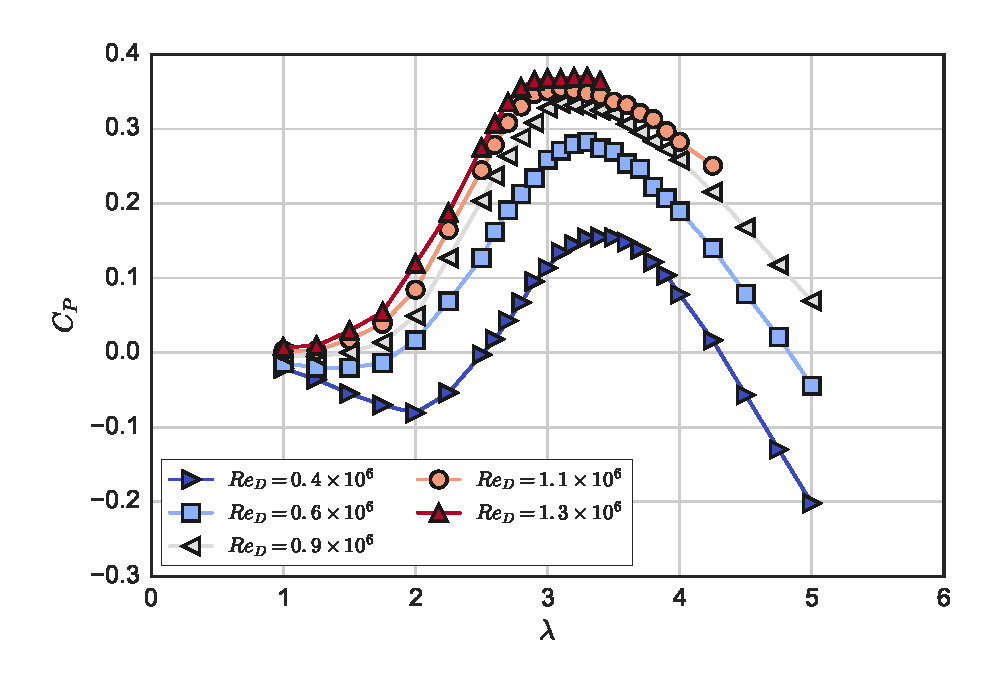
\includegraphics[width=\textwidth]{figures/cp_curves}
\caption{{\bf Power Coefficient Curves.}
Mean rotor power coefficient plotted versus mean tip speed ratio for multiple
Reynolds numbers.}
\label{cp-curves}
\end{figure}


\begin{figure}[h]
%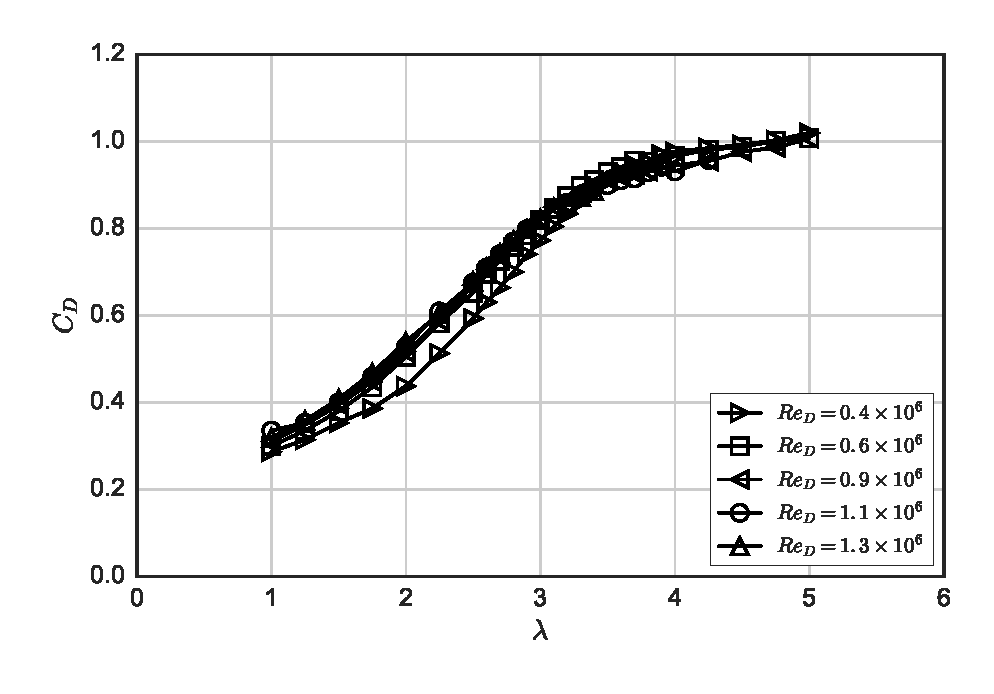
\includegraphics[width=\textwidth]{figures/cd_curves}
\caption{{\bf Drag Coefficient Curves.}
Mean rotor drag coefficient plotted versus mean tip speed ratio for multiple
Reynolds numbers.}
\label{cd-curves}
\end{figure}


\begin{figure}[h]
%\includegraphics[width=\textwidth]{figures/re_dep_cp}
\caption{{\bf Power Coefficient Reynolds Number Dependence.}
Power coefficient at $\lambda=3.1$ plotted versus Reynolds number.}
\label{cp-re-dep}
\end{figure}


\subsection*{Wake characteristics}

Nulla mi mi, venenatis sed ipsum varius, volutpat euismod diam. Proin rutrum vel
massa non gravida. Quisque tempor sem et dignissim rutrum. Lorem ipsum dolor sit
amet, consectetur adipiscing elit. Morbi at justo vitae nulla elementum commodo
eu id massa. In vitae diam ac augue semper tincidunt eu ut eros. Fusce fringilla
erat porttitor lectus cursus, vel sagittis arcu lobortis. Aliquam in enim
semper, aliquam massa id, cursus neque. Praesent faucibus semper libero.


\begin{figure}[h]
%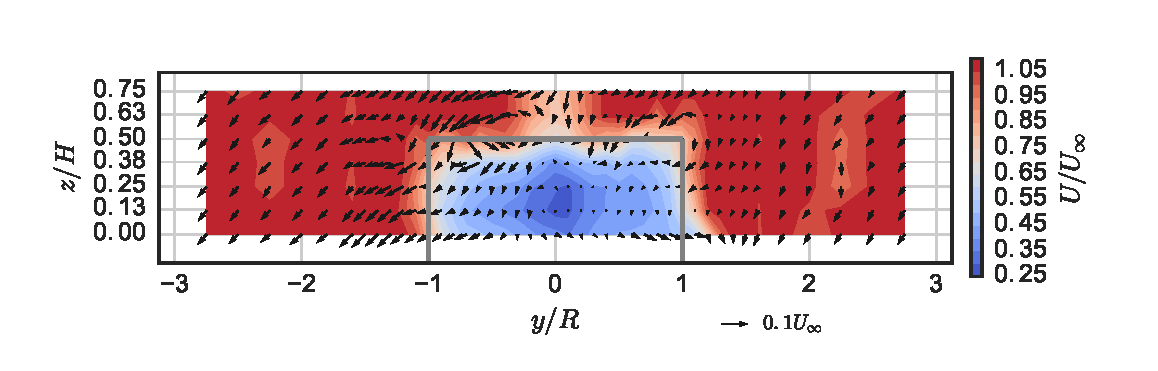
\includegraphics[width=\textwidth]{figures/meancontquiv}
\caption{{\bf Near-Wake Mean Velocity Field.}
Mean velocity field at 1 m downstream ($x/D=0.93$), $U_\infty=1.0$ m/s, and
$\lambda=3.1$.}
\label{meancontquiv}
\end{figure}


\begin{figure}[h]
%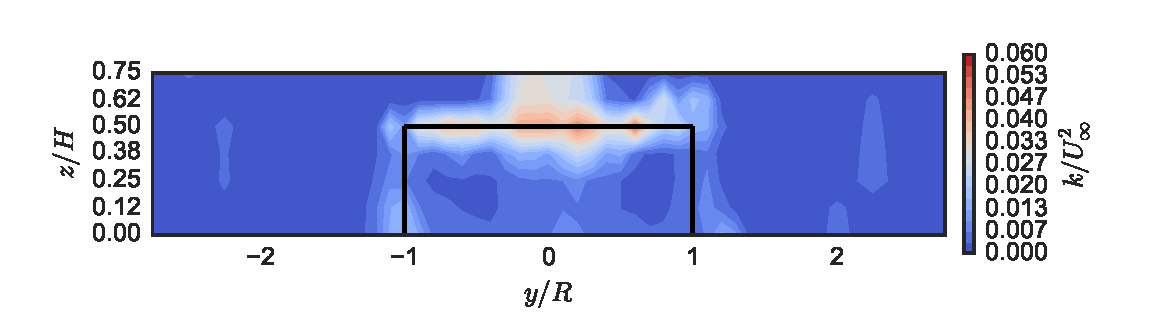
\includegraphics[width=\textwidth]{figures/k_contours}
\caption{{\bf Turbulence Kinetic Energy.}
Turbulence kinetic energy at 1 m downstream ($x/D=0.93$), $U_\infty=1.0$ m/s, and
$\lambda=3.1$.}
\label{kcont}
\end{figure}


% Please do not create a heading level below \subsection. For 3rd level
% headings, use \paragraph{}.
\subsection*{Subsection 1}
Nulla mi mi, venenatis sed ipsum varius, volutpat euismod diam. Proin rutrum vel
massa non gravida. Quisque tempor sem et dignissim rutrum. Lorem ipsum dolor sit
amet, consectetur adipiscing elit. Morbi at justo vitae nulla elementum commodo
eu id massa. In vitae diam ac augue semper tincidunt eu ut eros. Fusce fringilla
erat porttitor lectus cursus, vel sagittis arcu lobortis. Aliquam in enim
semper, aliquam massa id, cursus neque. Praesent faucibus semper libero.

\subsection*{Subsection 2}
\paragraph{3rd Level Heading.} Nulla mi mi, venenatis sed ipsum varius, volutpat
euismod diam. Proin rutrum vel massa non gravida. Quisque tempor sem et
dignissim rutrum. Lorem ipsum dolor sit amet, consectetur adipiscing elit. Morbi
at justo vitae nulla elementum commodo eu id massa. In vitae diam ac augue
semper tincidunt eu ut eros. Fusce fringilla erat porttitor lectus cursus, vel
sagittis arcu lobortis. Aliquam in enim semper, aliquam massa id, cursus neque.
Praesent faucibus semper libero.


\section*{Supporting Information}

% Include only the SI item label in the subsection heading. Use the \nameref{label} command to cite SI items in the text.
\subsection*{S1 Video}
\label{S1_Video}
{\bf Bold the first sentence.}  Maecenas convallis mauris sit amet sem ultrices
gravida. Etiam eget sapien nibh. Sed ac ipsum eget enim egestas ullamcorper nec
euismod ligula. Curabitur fringilla pulvinar lectus consectetur pellentesque.

\subsection*{S1 Text}
\label{S1_Text}
{\bf Lorem Ipsum.} Maecenas convallis mauris sit amet sem ultrices gravida.
Etiam eget sapien nibh. Sed ac ipsum eget enim egestas ullamcorper nec euismod
ligula. Curabitur fringilla pulvinar lectus consectetur pellentesque.

\subsection*{S1 Fig}
\label{S1_Fig}
{\bf Lorem Ipsum.} Maecenas convallis mauris sit amet sem ultrices gravida.
Etiam eget sapien nibh. Sed ac ipsum eget enim egestas ullamcorper nec euismod
ligula. Curabitur fringilla pulvinar lectus consectetur pellentesque.

\subsection*{S2 Fig}
\label{S2_Fig}
{\bf Lorem Ipsum.} Maecenas convallis mauris sit amet sem ultrices gravida.
Etiam eget sapien nibh. Sed ac ipsum eget enim egestas ullamcorper nec euismod
ligula. Curabitur fringilla pulvinar lectus consectetur pellentesque.

\subsection*{S1 Table}
\label{S1_Table}
{\bf Lorem Ipsum.} Maecenas convallis mauris sit amet sem ultrices gravida.
Etiam eget sapien nibh. Sed ac ipsum eget enim egestas ullamcorper nec euismod
ligula. Curabitur fringilla pulvinar lectus consectetur pellentesque.

\section*{Acknowledgments}
Cras egestas velit mauris, eu mollis turpis pellentesque sit amet. Interdum et
malesuada fames ac ante ipsum primis in faucibus. Nam id pretium nisi. Sed ac
quam id nisi malesuada congue. Sed interdum aliquet augue, at pellentesque quam
rhoncus vitae.

\nolinenumbers

% Compile your BiBTeX database using our plos2015.bst
% style file and paste the contents of your .bbl file
% here.
% 
\bibliography{library}


\end{document}

